During the long shutdown in 2014 ATLAS installed one of the first diamond pixel detectors - the \ac{DBM} - as an upgrade of the \ac{BCM}. Its purpose is to measure an instantaneous (bunch-by-bunch) luminosity and the bunch-by-bunch position of the beam spot. The \ac{DBM} consists of eight telescopes, four on each side of the \ac{IP}. Each of these telescopes comprises three detector planes. This adds tracking capability to the existing precise \ac{ToF} measurements of the original eight pad detectors of the \ac{BCM}. Using state-of-the-art pixel detectors based on the FE-I4B \ac{ROC} \cite{malte} increases the segmentation and the spatial resolution of the beam monitor and due to its projective geometry pointing towards the interaction region it can distinguish particles coming from collisions and background \cite{dbm}. The telescopes - six of which are built from \pcvd diamonds and two from silicon as reference - are positioned symmetrically around the beam pipe on both sides of the \ac{IP} and are shown in Figure \vref{dbm}. A total number of 45 diamonds with a thickness of \SI{500}{\micro\meter} were available for the project of which 18 were chosen for the detector.

\begin{figure}
	\centering
	\begin{subfigure}{.66\textwidth}
		\centering
		\vspace*{.05\textheight}
		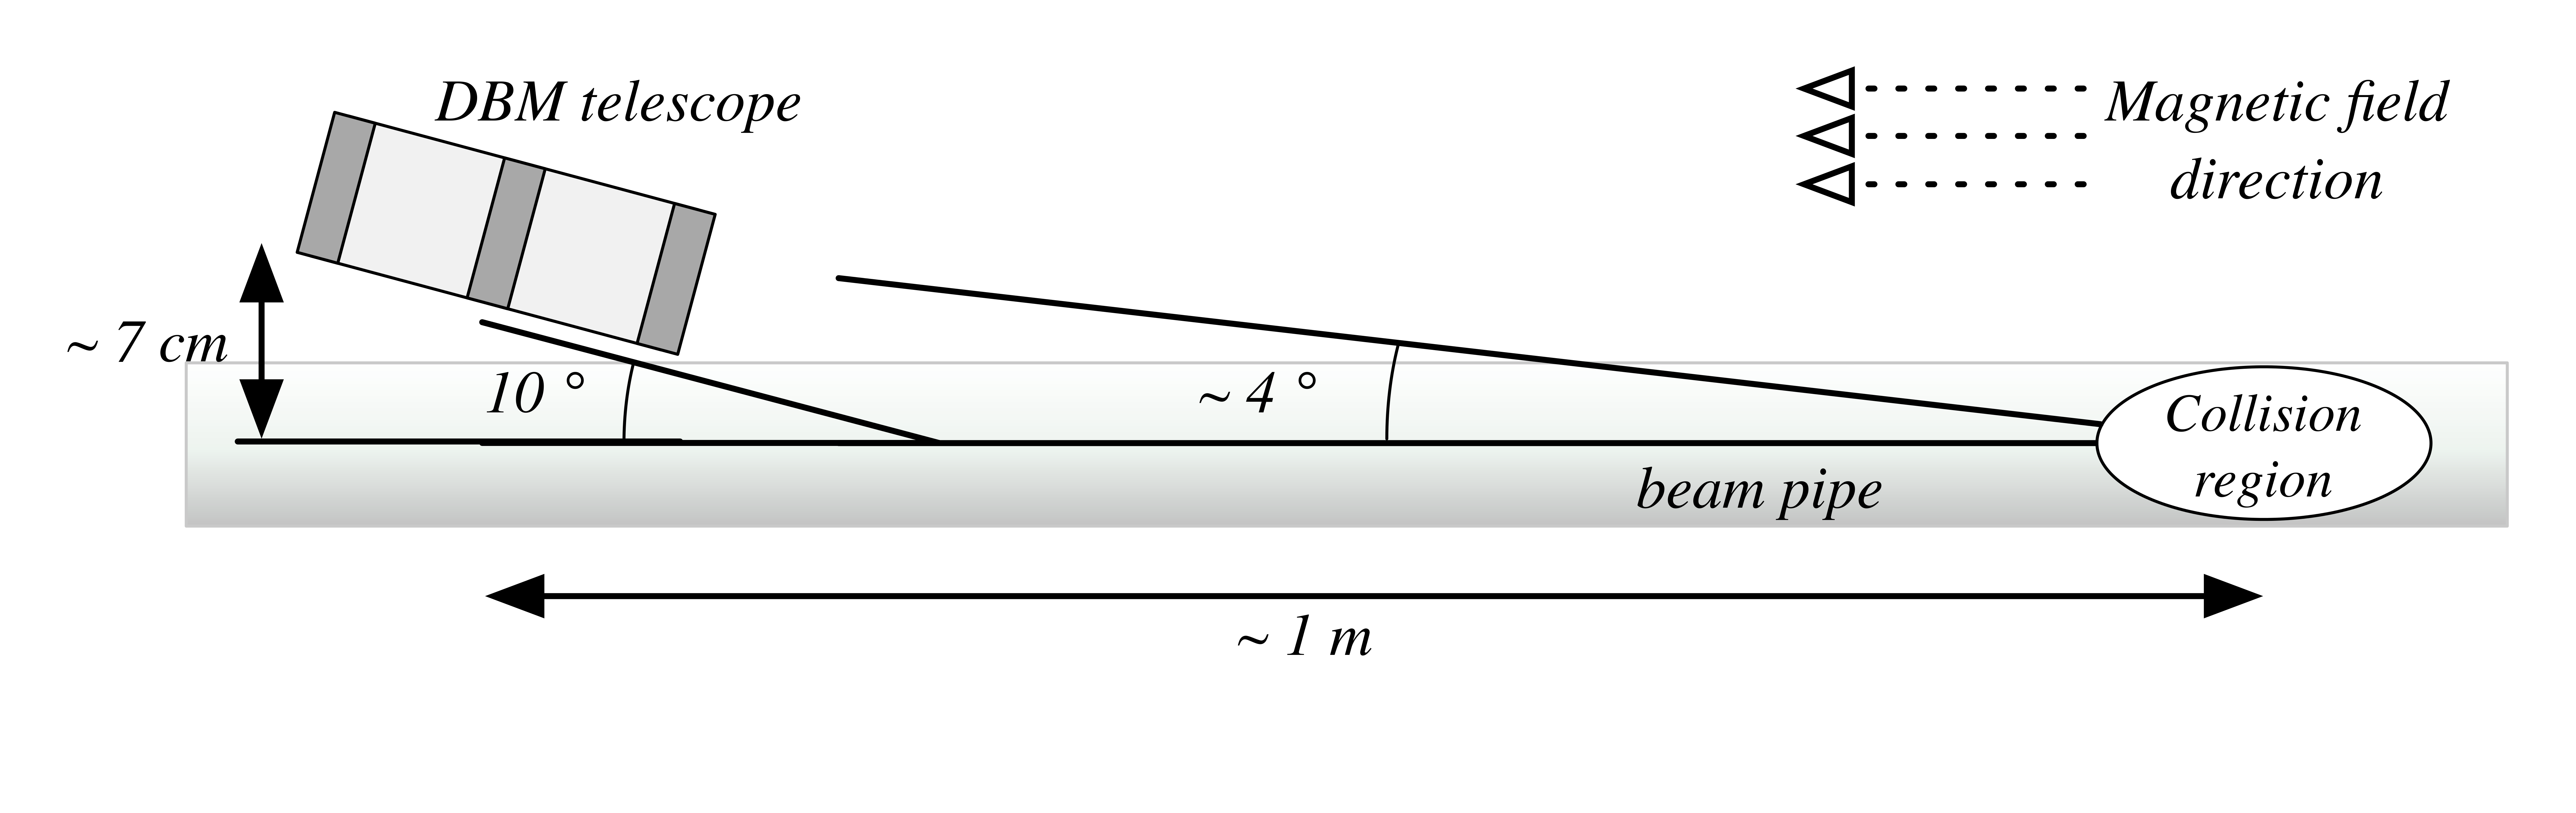
\includegraphics[height=.14\textheight]{dbm1.png}
		\vspace*{.02\textheight}
		\caption{positioning and alignment (from \cite{dbm})}
	\end{subfigure}
	\subfig[.33]{DBM2.png}{.23}{four mounted telescopes}
	\caption{The positioning of \ac{DBM} telescope around the beam pipe of the \ac{LHC}}
	\label{dbm}
\end{figure}

\noindent
% Shortly after the installation some of the modules broke (both silicon and diamond)and the \ac{DBM} became non-operational. Nevertheless 
The first results already show a clear discrimination between collision and background events as demonstrated in Figure \vref{dbmtrack}. During the shutdown of the \ac{LHC} in the beginning of 2017 the modules were recommissioned and are now a part of the ATLAS data taking.

\begin{figure}
	\centering
	\subfig{DBMTrack1.png}{.21}{longitudinal distance to the \ac{IP}}
	\subfig{DBMTrack2.png}{.21}{radial distance to the \ac{IP}}
	\caption{Reconstruction of tracks from three modules using the initial alignment.}
	\label{dbmtrack}
\end{figure}

% \noindent
% Du to the increasing particle fluence and excellent properties it is likely that diamond detectors become more popularin the future. The current research concentrates on 3D diamond detectors which will be described in section \vref{3D} as a possible candidate for the innermost tracking detectors of the \ac{LHC}. But there is also work towards an upgrade of the \ac{BCM} to the \ac{BCM}' which is designed to provide a fast (bunch-by-bunch) abort system for ATLAS as well as precise luminosity measurement for the \ac{HL-LHC}.